\documentclass[../ai_in_finance]{subfiles}
\usepackage[margin=1in]{geometry}
\usepackage{tikz}
\usetikzlibrary{positioning}
\usepackage{amsmath}
\usepackage{amssymb}
\usepackage{booktabs}
\usepackage{floatrow}
\usepackage{draftwatermark}

\SetWatermarkText{WSuo@Queensu.ca}
\SetWatermarkScale{1.4}
\SetWatermarkColor{gray!35}
\SetWatermarkAngle{45}

\usepackage{makeidx}
\makeindex

\begin{document}

\chapter{Financial Statements and Business Basics}

\section{Introduction}

Financial statements are the language through which firms communicate their economic position to investors, lenders, regulators, and managers. They are not merely accounting artifacts. They are structured summaries of how a business creates value, uses capital, and manages risk. For anyone working in finance, whether as an investor, analyst, trader, or data scientist, the ability to read and interpret financial statements is indispensable. A model may forecast returns or defaults, but it is useless without an understanding of the business context behind the numbers.

This chapter introduces the three core financial statements: the balance sheet, the income statement, and the cash flow statement. It explains how they fit together, why they differ, and how they can be used to reason about profitability, liquidity, solvency, and value creation. The chapter also works through a single running numerical example, a small fictional manufacturing firm, so that every ratio and concept can be tied to actual numbers rather than abstract definitions. The goal is not to turn the reader into an accountant, but to build the practical intuition needed to analyze firms in a way that is both financially sound and quantitatively useful.

Meridian Fabrication Inc., a fictional manufacturing firm, runs through the entire chapter as its central worked example: its balance sheet, income statement, and cash flow statement are built up section by section, then mined for liquidity, leverage, profitability, and efficiency ratios (Section~\ref{sec:ratios}), an Altman's Z-Score distress assessment, and a common-size restatement that makes its cost structure comparable across firm sizes. A second company, Solstice Robotics Inc. (Section~\ref{sec:solstice}), is introduced specifically for comparison, so that a ratio's meaning becomes clear by contrast rather than by definition alone: the same debt-to-equity ratio can signal prudence at one firm and fragility at another, depending on the business built around it.

This progression matters beyond the two companies themselves. The ratio toolkit built here is the same toolkit Chapter 9's credit scoring and Chapter 6's classification models eventually formalize statistically; Section~\ref{sec:valuation-connection} makes the link to Chapter 5's valuation models explicit, since a discounted-cash-flow model is only as trustworthy as the financial-statement forecasts feeding it; and the accounting-quality cautions raised late in the chapter, that reported numbers reflect choices and estimates, not just facts, are worth carrying into every later chapter that treats a financial statement's numbers as clean model inputs rather than as the product of a real, sometimes discretionary, reporting process.

\section{Why Financial Statements Matter}\index{Why Financial Statements Matter}

A firm is a system for converting resources into cash flows. It buys inputs, hires labor, invests in equipment, and sells products or services. In the process, it makes decisions about financing, operations, and strategy. Financial statements are the records that summarize these decisions. They allow stakeholders to ask essential questions: How much debt does the firm carry? Is it profitable? Is it generating enough cash to fund operations? What portion of the business is financed by owners versus lenders? Is growth coming from genuine operating improvement or from financial engineering?

These questions matter because finance is not only about price changes. It is also about the underlying economic reality of the firm. A stock can appear attractive because its price rises, but if the company is consuming cash and taking on excessive leverage, the apparent success may be fragile. Conversely, a firm with modest headline earnings may still be valuable if it produces durable cash flows and has strong competitive advantages. Financial statements help separate signal from noise.

In practice, the statements are analyzed together rather than in isolation. The balance sheet shows the firm's position at a point in time. The income statement shows performance over a period. The cash flow statement shows the movement of cash. Together, they provide a more complete picture than any single report could provide. Figure~\ref{fig:three_statements} sketches how the three statements relate to one another.

\begin{figure}[htbp]
\centering
\begin{lrbox}{\bookmeasuredbox}
    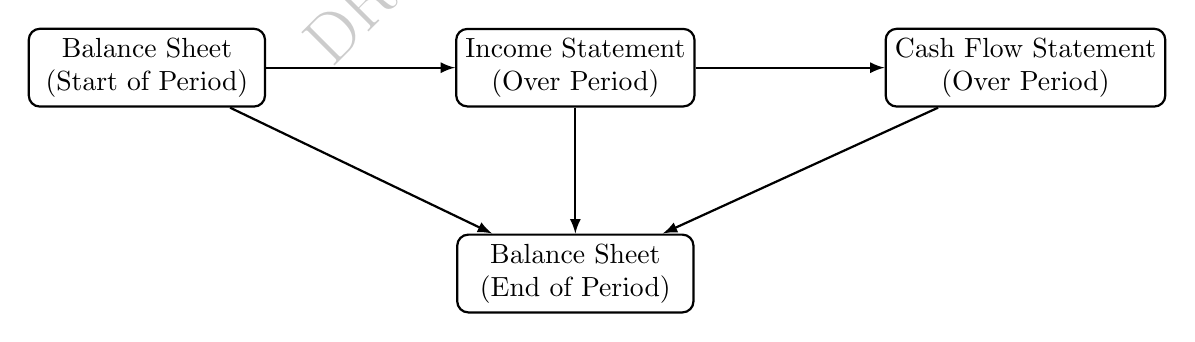
\begin{tikzpicture}[>=latex,thick,node distance=2.4cm]
        \node[draw,rounded corners,minimum width=3.0cm,minimum height=0.9cm,align=center] (bs1) {Balance Sheet\\(Start of Period)};
        \node[draw,rounded corners,minimum width=3.0cm,minimum height=0.9cm,right=of bs1,align=center] (is) {Income Statement\\(Over Period)};
        \node[draw,rounded corners,minimum width=3.0cm,minimum height=0.9cm,right=of is,align=center] (cf) {Cash Flow Statement\\(Over Period)};
        \node[draw,rounded corners,minimum width=3.0cm,minimum height=0.9cm,below=1.6cm of is,align=center] (bs2) {Balance Sheet\\(End of Period)};
        \draw[->] (bs1) -- (is);
        \draw[->] (is) -- (cf);
        \draw[->] (is) -- (bs2);
        \draw[->] (cf) -- (bs2);
        \draw[->] (bs1) -- (bs2);
    \end{tikzpicture}
\end{lrbox}
\ifdim\wd\bookmeasuredbox<0.65\linewidth
\setlength{\bookcapwidth}{0.65\linewidth}
\else
\setlength{\bookcapwidth}{\wd\bookmeasuredbox}
\fi
\ffigbox[\bookcapwidth]{
\usebox{\bookmeasuredbox}
}{
    \caption{The three statements are linked: the income statement and cash flow statement explain the change in the balance sheet from the start to the end of the period.}
    \label{fig:three_statements}
}
\end{figure}

\section{A Running Example: Meridian Fabrication\index{Meridian Fabrication Inc.} Inc.}\index{Meridian Fabrication Inc.}

To keep the discussion concrete, this chapter follows a single fictional company, Meridian Fabrication Inc., a small industrial parts manufacturer. All figures are in millions of dollars. Table~\ref{tab:meridian_bs} shows a simplified balance sheet at the end of two consecutive fiscal years, Table~\ref{tab:meridian_is} shows the income statement for the most recent year, and Table~\ref{tab:meridian_cf} shows the cash flow statement for the same year. These numbers are used throughout the chapter to illustrate ratios, forecasting, and the limits of reported figures.

\begin{table}[htbp]
\centering
\caption{Meridian Fabrication Inc. -- Balance Sheet (\$ millions)}
\label{tab:meridian_bs}
\begin{tabular}{lrr}
\toprule
 & Year 1 & Year 2 \\
\midrule
Cash and equivalents            & 12.0 & 9.0 \\
Accounts receivable             & 18.0 & 24.0 \\
Inventory                       & 22.0 & 30.0 \\
\textbf{Total current assets}   & \textbf{52.0} & \textbf{63.0} \\
Property, plant, and equipment (net) & 60.0 & 66.0 \\
\textbf{Total assets}           & \textbf{112.0} & \textbf{129.0} \\
\midrule
Accounts payable                & 14.0 & 17.0 \\
Short-term debt                 & 6.0  & 8.0 \\
\textbf{Total current liabilities} & \textbf{20.0} & \textbf{25.0} \\
Long-term debt                  & 40.0 & 50.0 \\
\textbf{Total liabilities}      & \textbf{60.0} & \textbf{75.0} \\
Shareholders' equity            & 52.0 & 54.0 \\
\textbf{Total liabilities and equity} & \textbf{112.0} & \textbf{129.0} \\
\bottomrule
\end{tabular}
\end{table}

\begin{table}[htbp]
\centering
\caption{Meridian Fabrication Inc. -- Income Statement, Year 2 (\$ millions)}
\label{tab:meridian_is}
\begin{tabular}{lr}
\toprule
Revenue                          & 150.0 \\
Cost of goods sold               & 96.0 \\
\textbf{Gross profit}            & \textbf{54.0} \\
Selling, general, and administrative expense & 30.0 \\
Depreciation and amortization    & 8.0 \\
\textbf{Operating income (EBIT)} & \textbf{16.0} \\
Interest expense                 & 4.0 \\
\textbf{Pretax income}           & \textbf{12.0} \\
Taxes (25\%)                     & 3.0 \\
\textbf{Net income}              & \textbf{9.0} \\
\bottomrule
\end{tabular}
\end{table}

\begin{table}[htbp]
\centering
\caption{Meridian Fabrication Inc. -- Cash Flow Statement, Year 2 (\$ millions)}
\label{tab:meridian_cf}
\begin{tabular}{lr}
\toprule
Net income                                & 9.0 \\
$+$ Depreciation and amortization         & 8.0 \\
$-$ Increase in accounts receivable       & 6.0 \\
$-$ Increase in inventory                 & 8.0 \\
$+$ Increase in accounts payable          & 3.0 \\
\textbf{Cash flow from operations}        & \textbf{6.0} \\
Capital expenditures                      & 14.0 \\
\textbf{Cash flow from investing}         & \textbf{$-$14.0} \\
Net new debt issued                       & 12.0 \\
Dividends paid                            & 7.0 \\
\textbf{Cash flow from financing}         & \textbf{5.0} \\
\textbf{Net change in cash}               & \textbf{$-$3.0} \\
\bottomrule
\end{tabular}
\end{table}

Notice, as a first observation, that Meridian's net income of \$9.0 million looks respectable, but cash flow from operations is only \$6.0 million, and after \$14.0 million of capital expenditures, the firm actually burned cash and had to raise \$12.0 million of new debt just to keep its cash balance from falling further. This is exactly the type of discrepancy between accounting profit and cash generation that financial statement analysis is designed to surface, and it will recur throughout the chapter.

\section{The Balance Sheet}\index{Balance Sheet}

The balance sheet is a snapshot of a firm's resources and claims at a specific date. It is governed by a simple accounting identity:

\begin{equation*}
\text{Assets} = \text{Liabilities} + \text{Equity}.
\end{equation*}

Assets are what the firm owns or controls. They include cash, receivables, inventories, property, plant and equipment, intangible assets, and other resources expected to generate future benefit. Liabilities are obligations the firm owes to others, such as loans, accounts payable, or taxes payable. Equity is the residual interest of owners after liabilities are subtracted from assets. In Table~\ref{tab:meridian_bs}, this identity holds in both years: \$112.0 million of assets equal \$60.0 million of liabilities plus \$52.0 million of equity in Year 1, and \$129.0 million equal \$75.0 million plus \$54.0 million in Year 2.

The balance sheet matters because it reveals the firm's financial structure. A firm with large cash reserves and modest debt is often more resilient than a firm with high leverage and weak liquidity. A firm with significant intangible assets may appear valuable in the market, but those assets may be harder to liquidate if the company encounters distress. A firm with high inventory levels may face operational risk if demand falls unexpectedly. Meridian's inventory grew from \$22.0 million to \$30.0 million, a 36\% increase, while revenue is discussed below; comparing the growth rate of inventory to the growth rate of sales is one of the simplest early-warning checks an analyst performs.

The balance sheet can be analyzed along several dimensions. One is liquidity, which concerns the firm's ability to meet short-term obligations. Another is capital structure, which concerns the mix of debt and equity financing. A third is asset quality, which concerns whether the reported assets are likely to generate value. Financial analysts commonly compute ratios such as current assets divided by current liabilities, debt divided by equity, and long-term debt relative to total assets. These ratios provide a first pass at understanding the firm's financial position and are computed explicitly for Meridian in Section~\ref{sec:ratios}.

\section{The Income Statement}\index{Income Statement}

The income statement summarizes revenues, expenses, and profit over a period such as a quarter or a year. It begins with revenue, which is the amount earned from selling goods or services. From revenue, the firm subtracts costs of goods sold and operating expenses to arrive at operating profit, often called earnings before interest and taxes (EBIT). Further deductions for interest and taxes lead to net income, which is often the headline figure quoted in the media.

For Meridian, revenue of \$150.0 million minus cost of goods sold of \$96.0 million yields gross profit of \$54.0 million, a gross margin of
\begin{equation*}
\text{Gross margin} = \frac{54.0}{150.0} = 36.0\%.
\end{equation*}
After subtracting SG\&A (\$30.0 million) and depreciation (\$8.0 million), operating income is \$16.0 million, an operating margin of
\begin{equation*}
\text{Operating margin} = \frac{16.0}{150.0} = 10.7\%.
\end{equation*}
After \$4.0 million of interest expense and \$3.0 million of taxes (a 25\% rate applied to \$12.0 million of pretax income), net income is \$9.0 million, a net margin of $9.0/150.0 = 6.0\%$.

Although net income is widely reported, it should not be interpreted mechanically. Accounting profit can be influenced by depreciation, amortization, one-time gains or losses, and estimates of reserves and provisions. These choices can affect the apparent profitability of a firm. For this reason, analysts often look beyond net income to operating income, adjusted earnings, and cash-based measures of performance.

Profitability is central to valuation. Investors care about whether the firm can earn returns above its cost of capital. A company may report growth in sales, but if margins are declining and competition is intensifying, future value may be under pressure. Profitability analysis therefore examines gross margin, operating margin, and net margin together with their trend over time, not just their level in a single year.

One further profitability measure is worth introducing alongside these three margins because of how frequently it appears in valuation practice: EBITDA\index{EBITDA}, earnings before interest, taxes, depreciation, and amortization, computed by adding depreciation and amortization back to operating income. For Meridian, $\text{EBITDA} = 16.0 + 8.0 = \$24.0$ million, an EBITDA margin of $24.0/150.0 = 16.0\%$. EBITDA is popular specifically because it strips out depreciation and amortization, non-cash charges that can vary substantially across firms depending on their accounting choices and asset age, making it easier to compare operating performance across companies with different capital structures and depreciation schedules.
It is not a substitute for free cash flow, since it ignores both capital expenditures and working-capital changes, both of which Meridian's own numbers show are large enough to turn a profitable-looking income statement into a cash-consuming year; but as a cross-sectional comparison tool, and as the denominator of the EV/EBITDA valuation multiple used throughout Chapter 5, it is worth computing routinely alongside gross, operating, and net margin.

\section{The Cash Flow Statement}\index{Cash Flow Statement}
\label{sec:cash-flow-statement}

The cash flow statement is often the most informative statement for understanding financial health. Cash is the ultimate resource that keeps a business alive. A company can report positive profits and still face liquidity problems if cash is tied up in inventory, receivables, or capital spending. The cash flow statement shows how cash is generated and used in three major activities: operating, investing, and financing.

Operating cash flow reflects cash generated from the core business. It starts from net income and adjusts for non-cash items (such as adding back depreciation) and for changes in working-capital accounts. Investing cash flow reflects purchases and sales of long-term assets, primarily capital expenditures. Financing cash flow reflects borrowing, repayments, dividends, and equity issuance. Table~\ref{tab:meridian_cf} shows this decomposition for Meridian: operating cash flow of \$6.0 million, investing cash flow of $-\$14.0$ million, and financing cash flow of \$5.0 million, which together produce a net decrease in cash of \$3.0 million, consistent with the cash balance falling from \$12.0 million to \$9.0 million on the balance sheet.

A particularly important concept is free cash flow\index{Free Cash Flow (FCF)}, typically defined as
\begin{equation*}
\text{Free cash flow} = \text{Cash flow from operations} - \text{Capital expenditures}.
\end{equation*}
For Meridian, free cash flow in Year 2 is $6.0 - 14.0 = -\$8.0$ million. This single number tells a sharper story than net income alone: despite reporting a \$9.0 million profit, Meridian generated negative \$8.0 million of free cash flow and had to borrow to cover the shortfall. Free cash flow is closely related to valuation because firms that generate consistent free cash flow can support dividends, debt repayment, or reinvestment without external financing. Many valuation frameworks explicitly use free cash flows rather than accounting earnings because the latter can be distorted by non-cash charges and discretionary accounting choices.

\section{Working Capital and Liquidity}\index{Working Capital and Liquidity}

Liquidity refers to the ability of a firm to meet short-term obligations. It is one of the clearest indicators of short-run financial health. A business that cannot pay suppliers, employees, or creditors on time may face operational disruption even if the long-term outlook is strong. Analysts therefore pay close attention to current assets, current liabilities, and the cycle of converting inventory and receivables into cash.

Working capital is defined as
\begin{equation*}
\text{Working capital} = \text{Current assets} - \text{Current liabilities}.
\end{equation*}
For Meridian, working capital rose from $52.0 - 20.0 = \$32.0$ million in Year 1 to $63.0 - 25.0 = \$38.0$ million in Year 2. On its own this looks like a healthy increase in resources, but combined with the cash flow statement it is clear that most of this increase is simply cash trapped in receivables and inventory rather than cash sitting in the bank. Too little working capital can cause distress, while too much may indicate inefficiency or, as in Meridian's case, a buildup that has not yet been converted back into cash.

In practice, working capital is actively managed, not just measured after the fact. A treasury or finance team can accelerate collections by offering early-payment discounts to customers, negotiate longer payment terms with suppliers, or use inventory management techniques such as just-in-time ordering to reduce the amount of cash tied up in stock at any given time. Each of these levers maps directly onto one of the three components of the cash conversion cycle computed below: 
shortening DSO (days sales outstanding) through faster collections, lengthening DPO (days payable outstanding) through supplier negotiation, or shortening DIO (days inventory outstanding) through leaner
 inventory management. Working capital financing, such as a revolving credit facility sized specifically to bridge 
the gap between paying suppliers and collecting from customers, is also common precisely because this gap, as Meridian's 
cash flow statement demonstrates, can consume substantial cash even for a fundamentally healthy and growing business.

The cash conversion cycle\index{Cash Conversion Cycle} is a useful way to quantify this. It is commonly expressed as
\begin{equation*}
\text{Cash conversion cycle} = \text{DIO} + \text{DSO} - \text{DPO},
\end{equation*}
where DIO  measures how long inventory sits before being sold, DSO  measures how long it takes to collect receivables after a sale,
and DPO  measures how long the firm takes to pay its own suppliers. COGS is cost of goods sold, the direct cost, materials, direct labor, and manufacturing overhead, of producing whatever a firm actually sold during the period, already introduced earlier in this chapter as the amount subtracted from revenue to arrive at gross profit.

DIO and DPO divide by COGS rather than revenue for a specific reason: inventory and accounts payable are both carried on the balance sheet at their cost to the firm, not at the higher price a customer eventually pays, so matching them against COGS, itself a cost-basis figure, keeps the ratio's numerator and denominator on the same footing.
DSO, by contrast, divides accounts receivable, which is recorded at the amount actually billed to the customer, by revenue, the corresponding billed-price figure; using COGS for DSO or revenue for DIO and DPO would quietly mix cost-basis and price-basis quantities in the same ratio. Using average balances and a 365-day year,
\begin{align*}
\text{DIO} &= \frac{\text{Inventory}}{\text{COGS}} \times 365 = \frac{30.0}{96.0}\times 365 \approx 114 \text{ days}, \\
\text{DSO} &= \frac{\text{Accounts receivable}}{\text{Revenue}} \times 365 = \frac{24.0}{150.0}\times 365 \approx 58 \text{ days}, \\
\text{DPO} &= \frac{\text{Accounts payable}}{\text{COGS}} \times 365 = \frac{17.0}{96.0}\times 365 \approx 65 \text{ days}.
\end{align*}
Rounding each component to the nearest day before summing gives $114 + 58 - 65 = 107$ days, but computing the cycle from the unrounded day-counts gives $114.06 + 58.40 - 64.64 \approx 107.8$, which rounds to 108 days; the one-day gap between the two is purely a rounding artifact from summing already-rounded intermediate figures, a small but instructive reminder to carry full precision through a multi-step calculation and round only the final answer. Either way, Meridian's cash is tied up in the operating cycle for roughly three and a half months before it returns to the firm. A shorter cycle is generally better because it means the firm can recycle cash more quickly and rely less on external financing. The cycle can be improved through better inventory management, faster collections, or more favorable supplier terms, and it is exactly the kind of quantity that a data-driven monitoring system can track continuously across many firms or product lines.

\section{Leverage and Solvency}\index{Leverage and Solvency}

Leverage refers to the extent to which a firm uses debt financing. Debt can be attractive because it is often cheaper than equity and interest expenses may be tax-deductible. However, leverage also increases financial risk. If the firm's cash flows are volatile, debt can become burdensome and may force restructuring or bankruptcy.

Solvency is the ability of a firm to meet its long-term obligations. Analysts examine leverage ratios such as debt-to-equity,
\begin{equation*}
\text{Debt-to-equity} = \frac{\text{Total debt}}{\text{Shareholders' equity}},
\end{equation*}
and interest coverage,
\begin{equation*}
\text{Interest coverage} = \frac{\text{EBIT}}{\text{Interest expense}}.
\end{equation*}
For Meridian in Year 2, total debt is short-term debt plus long-term debt, $8.0 + 50.0 = \$58.0$ million, against equity of \$54.0 million, giving a debt-to-equity ratio of $58.0/54.0 \approx 1.07$: the firm is financed with slightly more debt than equity. Interest coverage is $16.0/4.0 = 4.0$, meaning operating income covers interest expense four times over. A coverage ratio of 4.0 is generally considered comfortable, but the trend matters: if debt continues to grow faster than operating income, coverage will fall and the firm's cushion against a bad year will shrink.

Leverage is not inherently good or bad. It depends on the firm's business model, cash-flow stability, and access to financing. A utility can often carry significant debt because its revenues are stable. A startup in a volatile industry may be unable to support much debt. The key is understanding whether leverage amplifies the firm's strengths or magnifies its weaknesses, and for Meridian, the fact that new debt was needed to fund a cash shortfall driven by working-capital growth is a signal worth investigating rather than ignoring.

\section{Sector-Specific Considerations in Ratio Analysis}\index{Sector-Specific Considerations in Ratio Analysis}

The chapter has repeatedly warned that ratios must be interpreted in context, and it is worth being specific about what that context looks like across a few contrasting industries, since a large-scale, cross-sectional financial model cannot apply a single set of thresholds to every firm it scores.

Banks and other financial institutions are the most extreme example. A bank's balance sheet consists mostly of financial assets (loans) funded mostly by financial liabilities (deposits), so a debt-to-equity ratio that would signal extreme distress for an industrial firm like Meridian, often 8 or 10 times equity, is routine and expected for a bank, whose entire business model is to hold a leveraged portfolio of loans. Standard liquidity ratios such as the current ratio are similarly not meaningful for banks, since a bank's balance sheet is not organized around a current/non-current distinction in the same way; regulators instead impose bank-specific capital and liquidity ratios, some of which were introduced in the Basel III\index{Basel Accords} discussion of Chapter 3.

Capital-intensive industries such as utilities, airlines, and telecommunications typically carry substantial long-term debt and correspondingly low interest coverage relative to a company like Solstice, precisely because their revenues are relatively stable and predictable (regulated utility rates, contracted infrastructure usage), which allows them to service more debt safely than a firm with volatile, uncertain cash flows. A debt-to-equity ratio of 1.5 might be unremarkable for a regulated utility but alarming for an unproven technology startup with the same ratio.

Asset-light service and technology businesses, more like Solstice than Meridian, often carry little debt, hold significant cash balances, and derive most of their value from intangible assets, customer relationships, brand, intellectual property, that may not appear as a large balance sheet line item at all under conventional accounting. This is one reason market-based valuation multiples (Chapter 5) are often used alongside, or instead of, book-value-based ratios for such firms: the balance sheet may substantially understate the economic assets actually driving the business.

The practical implication for any model built across many firms is that ratios should typically be compared within a sector or peer group rather than against a single universal threshold, and that sector membership itself, along with variables like capital intensity, is often a useful feature to include directly in a predictive model rather than something to control for only informally.

This has a direct, quantitative consequence for a distress score like Altman's Z$'$: a formula whose coefficients were estimated primarily on manufacturing and industrial firms will systematically misclassify a bank, whose debt-to-equity ratio, and therefore $X_4$, would sit far below any threshold intended for an industrial company, even for a perfectly healthy bank. Neither Meridian's Z$'$-score of 2.41 nor Solstice's 4.33, computed earlier in this chapter, would be directly comparable to a Z$'$-score computed for a bank or a capital-intensive utility using the same coefficients, which is exactly why credit-scoring models built for a specific sector, such as the bank-focused credit risk material in Chapter 9, are estimated on sector-specific data rather than reusing a general-purpose formula like Altman's across every industry.

\section{How Firms Create Value}\index{How Firms Create Value}

Suppose a firm doubles its revenue and its balance sheet over five years, yet its shareholders end up no wealthier than if the firm had stayed the same size. Growth alone, it turns out, says nothing about whether a firm is actually creating value, because growth has to be paid for with capital, and that capital has a cost, whether it comes from lenders demanding interest or shareholders demanding a competitive return on their investment. A firm creates value only when it earns returns on invested capital that exceed the cost of that capital; if a company invests in projects that earn more than the required return, value is created, and if it invests in projects that earn less than the required return, value is destroyed no matter how much bigger the firm gets in the process. This is one of the most important ideas in corporate finance, and a common way to express it is through economic profit\index{Economic Profit},
\begin{equation*}
\text{Economic profit} = \text{Invested capital} \times (\text{ROIC} - \text{WACC}),
\end{equation*}
where ROIC is the return on invested capital and WACC is the weighted average cost of capital. A simple value-creation diagram is shown in Figure~\ref{fig:value_creation}.

\begin{figure}[htbp]
\centering
\begin{lrbox}{\bookmeasuredbox}
    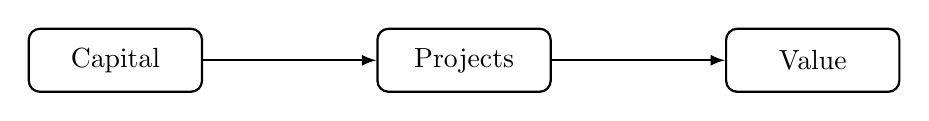
\begin{tikzpicture}[>=latex,thick,node distance=2.2cm]
        \node[draw,rounded corners,minimum width=2.2cm,minimum height=0.8cm] (capital) {Capital};
        \node[draw,rounded corners,minimum width=2.2cm,minimum height=0.8cm,right=of capital] (project) {Projects};
        \node[draw,rounded corners,minimum width=2.2cm,minimum height=0.8cm,right=of project] (value) {Value};
        \draw[->] (capital) -- (project);
        \draw[->] (project) -- (value);
    \end{tikzpicture}
\end{lrbox}
\ifdim\wd\bookmeasuredbox<0.65\linewidth
\setlength{\bookcapwidth}{0.65\linewidth}
\else
\setlength{\bookcapwidth}{\wd\bookmeasuredbox}
\fi
\ffigbox[\bookcapwidth]{
\usebox{\bookmeasuredbox}
}{
    \caption{A firm generates value when its projects earn a return above the cost of capital.}
    \label{fig:value_creation}
}
\end{figure}

This idea links financial statements to valuation. A firm that generates high returns on capital and reinvests profitably can compound value over time. A firm that earns low returns and uses excessive leverage may appear large but create little wealth. Data scientists working in finance often use accounting and market data together to evaluate such patterns. A predictive model may forecast changes in revenue, but an analyst must still ask whether those changes translate into durable value creation.

The concept also explains why growth is not always beneficial. Growth can be valuable when it is tied to profitable reinvestment. Growth can be harmful when it requires large amounts of capital with weak expected returns. Meridian grew its balance sheet from \$112.0 million to \$129.0 million, a 15\% increase, while free cash flow turned negative; whether this growth is value-creating depends on whether the additional invested capital will eventually generate returns above its cost, which is a question the statements alone cannot answer but strongly motivate asking.

The statements alone cannot supply a cost of capital, but they can supply everything else this calculation needs. Meridian's invested capital, the sum of its interest-bearing debt and equity, is $\$58.0 + \$54.0 = \$112.0$ million (Table~\ref{tab:meridian_bs}), and its after-tax operating profit, or net operating profit after tax (NOPAT), is $\text{EBIT} \times (1 - \text{tax rate}) = 16.0 \times 0.75 = \$12.0$ million. This gives
\begin{equation*}
\text{ROIC} = \frac{\text{NOPAT}}{\text{Invested capital}} = \frac{12.0}{112.0} \approx 10.7\%.
\end{equation*}
If Meridian's weighted average cost of capital, estimated using the methods of Chapter 5, were $8\%$, its economic profit would be $112.0 \times (0.107 - 0.08) \approx \$3.0$ million: modestly positive, meaning Meridian is creating a small amount of value on top of its cost of capital despite the cash-flow strain documented earlier in this chapter. This is an important, if initially counterintuitive, distinction: a firm can be a genuine (if marginal) value creator by this economic-profit measure while simultaneously burning cash and increasing leverage, because ROIC versus WACC answers whether capital is being deployed productively, while free cash flow answers a different question, whether the firm is generating or consuming cash in the short run. A machine learning model trained to predict ``financial health'' from statement data needs to be clear about which of these two, economically distinct, questions it is actually answering.

\section{Common Financial Ratios and What They Reveal}\index{Common Financial Ratios and What They Reveal}
\label{sec:ratios}

Financial ratios are one of the simplest ways to convert raw statements into interpretable measures. They help analysts compare firms, track trends over time, and identify areas of concern. Ratios can be grouped into categories such as profitability, liquidity, efficiency, solvency, and valuation. Table~\ref{tab:ratio_summary} collects the main ratio families together with their formulas and Meridian's Year 2 values.

\begin{table}[htbp]
\centering
\caption{Summary of common financial ratios, applied to Meridian, Year 2}
\label{tab:ratio_summary}
\begin{tabular}{p{3.4cm}p{5.4cm}r}
\toprule
Ratio & Formula & Meridian Value \\
\midrule
Current ratio & Current assets / Current liabilities & $63.0/25.0 = 2.52$ \\
Quick ratio & (Current assets $-$ Inventory) / Current liabilities & $33.0/25.0 = 1.32$ \\
Gross margin & Gross profit / Revenue & $54.0/150.0 = 36.0\%$ \\
Operating margin & EBIT / Revenue & $16.0/150.0 = 10.7\%$ \\
Net margin & Net income / Revenue & $9.0/150.0 = 6.0\%$ \\
Debt-to-equity & Total debt / Equity & $58.0/54.0 = 1.07$ \\
Interest coverage & EBIT / Interest expense & $16.0/4.0 = 4.0$ \\
Asset turnover & Revenue / Total assets & $150.0/129.0 = 1.16$ \\
Return on equity (ROE) & Net income / Equity & $9.0/54.0 = 16.7\%$ \\
\bottomrule
\end{tabular}
\end{table}

The current ratio of 2.52 and quick ratio of 1.32 suggest that, on paper, Meridian has ample short-term resources to cover its current liabilities. Yet this is precisely where the earlier cash flow analysis adds crucial nuance: much of the current assets are tied up in slow-moving inventory and receivables rather than cash, and the firm's actual cash balance fell during the year. A ratio computed from a single balance sheet date can look comfortable while masking a deteriorating cash trajectory, which is why ratios are always more informative when read together with the cash flow statement and their own historical trend.

A particularly useful decomposition is the DuPont identity\index{DuPont Identity}, which breaks return on equity into three economically distinct drivers:
\begin{equation*}
\text{ROE} = \underbrace{\frac{\text{Net income}}{\text{Revenue}}}_{\text{Net margin}} \times \underbrace{\frac{\text{Revenue}}{\text{Total assets}}}_{\text{Asset turnover}} \times \underbrace{\frac{\text{Total assets}}{\text{Equity}}}_{\text{Equity multiplier}}.
\end{equation*}
For Meridian, $\text{Net margin} = 6.0\%$, $\text{Asset turnover} = 1.16$, and the equity multiplier is $129.0/54.0 = 2.39$. Multiplying these together, $0.060 \times 1.16 \times 2.39 \approx 16.6\%$, which matches the directly computed ROE of 16.7\% up to rounding. The value of this decomposition is diagnostic: it shows that Meridian's ROE is being driven substantially by leverage (an equity multiplier above 2) rather than by unusually high margins or asset efficiency. Two firms can report the same ROE for very different, and not equally sustainable, reasons, and the DuPont breakdown is the standard tool for telling them apart.

The three-factor version above bundles taxes, interest, and core operating profitability together inside a single ``net margin'' term, which hides whether a firm's margin is being driven by its actual operations or merely by a favorable tax or financing outcome. The five-factor extended DuPont identity splits net margin further,
\begin{equation*}
\text{ROE} = \underbrace{\frac{\text{Net income}}{\text{Pretax income}}}_{\text{Tax burden}} \times \underbrace{\frac{\text{Pretax income}}{\text{EBIT}}}_{\text{Interest burden}} \times \underbrace{\frac{\text{EBIT}}{\text{Revenue}}}_{\text{Operating margin}} \times \text{Asset turnover} \times \text{Equity multiplier},
\end{equation*}
isolating exactly how much of net margin survives taxation and interest expense before operating profitability is even considered. For Meridian, the tax burden is $9.0/12.0 = 0.75$ (the firm retains $75\%$ of pretax income after taxes, consistent with the $25\%$ tax rate used throughout this chapter), the interest burden is $12.0/16.0 = 0.75$ (the firm retains $75\%$ of EBIT after interest expense), and the operating margin is $16.0/150.0 \approx 10.7\%$, exactly the operating margin already computed in Section~\ref{sec:ratios}. Multiplying all five factors,
\begin{equation*}
0.75 \times 0.75 \times 0.107 \times 1.163 \times 2.389 \approx 16.7\%,
\end{equation*}
matches the directly computed ROE exactly. The diagnostic value of the extra split is immediate: Meridian's two burden ratios are identical at $0.75$, meaning taxes and interest expense are eroding profitability by the same proportion, but a firm with, say, a much lower interest burden (heavily levered, paying substantial interest) and a high tax burden would show an identical three-factor net margin to Meridian while having a completely different underlying cost structure, a distinction only the five-factor decomposition, not the three-factor one, can actually surface.

Liquidity ratios such as the current ratio and quick ratio assess how easily a firm can meet short-term obligations. Efficiency ratios such as inventory turnover and receivables turnover reveal how quickly the firm converts resources into cash. Solvency ratios such as debt-to-equity and interest coverage reveal how vulnerable the firm is to financial distress. Valuation ratios such as price-to-earnings and price-to-book are often used by investors to compare market expectations with fundamental performance, though they require market price data that goes beyond the statements themselves.

The usefulness of ratios depends on context. A high leverage ratio may be acceptable for a stable utility but dangerous for a startup with volatile cash flows. A low inventory turnover ratio may indicate weak sales or poor inventory management, but in some sectors it may simply reflect a strategy of high service levels. Ratios are therefore best used as starting points for a conversation about the business, not as final judgments in themselves.

\section{A Second Company for Comparison: Solstice Robotics Inc.}\index{Solstice Robotics Inc.}
\label{sec:solstice}

Ratios are most informative in relative terms, compared across firms or across time, not in isolation. To make this concrete, consider a second fictional company, Solstice Robotics Inc., a faster-growing, less capital-intensive firm, with the Year 2 figures in Table~\ref{tab:solstice}.

\begin{table}[htbp]
\centering
\caption{Solstice Robotics Inc. -- Summary Financials, Year 2 (\$ millions)}
\label{tab:solstice}
\begin{tabular}{lr}
\toprule
Cash and equivalents & 40.0 \\
Accounts receivable & 20.0 \\
Inventory & 10.0 \\
\textbf{Total current assets} & \textbf{70.0} \\
Property, plant, and equipment (net) & 30.0 \\
\textbf{Total assets} & \textbf{100.0} \\
\midrule
Accounts payable & 15.0 \\
Long-term debt & 10.0 \\
\textbf{Total liabilities} & \textbf{25.0} \\
Shareholders' equity & 75.0 \\
\midrule
Revenue & 120.0 \\
Cost of goods sold & 48.0 \\
SG\&A & 40.0 \\
Depreciation and amortization & 5.0 \\
Interest expense & 1.0 \\
Net income & 19.5 \\
\bottomrule
\end{tabular}
\end{table}

Table~\ref{tab:comparison} places Meridian and Solstice side by side on the same ratios computed in Table~\ref{tab:ratio_summary}.

\begin{table}[htbp]
\centering
\caption{Meridian versus Solstice, Year 2}
\label{tab:comparison}
\begin{tabular}{lrr}
\toprule
Ratio & Meridian & Solstice \\
\midrule
Current ratio & 2.52 & 4.67 \\
Quick ratio & 1.32 & 4.00 \\
Gross margin & 36.0\% & 60.0\% \\
Operating margin & 10.7\% & 22.5\% \\
Net margin & 6.0\% & 16.25\% \\
Debt-to-equity & 1.07 & 0.13 \\
Interest coverage & 4.0 & 27.0 \\
Return on equity & 16.7\% & 26.0\% \\
\bottomrule
\end{tabular}
\end{table}

Solstice's ROE of 26\% is higher than Meridian's 16.7\%, but the DuPont identity from Section~\ref{sec:ratios} reveals that the two firms get there in opposite ways. Applying the same decomposition to Solstice: net margin $16.25\%$, asset turnover $120.0/100.0 = 1.20$, and equity multiplier $100.0/75.0 = 1.33$, so $0.1625 \times 1.20 \times 1.33 \approx 26.0\%$, matching directly.

Solstice's high ROE is driven almost entirely by superior margins (16.25\% net margin versus Meridian's 6.0\%), with very little help from leverage (an equity multiplier of 1.33 versus Meridian's 2.39). Meridian, by contrast, achieves a respectable but lower ROE mostly \emph{because} of leverage. An analyst, or a machine learning model trained naively on ROE alone, would rank the two firms similarly on this one statistic despite their financial structures, and therefore their risk profiles, being almost opposite; this is precisely the kind of distinction the DuPont decomposition exists to surface, and precisely the kind of nuance a single summary ratio can hide.

\section{Common-Size Statements}\index{Common-Size Statements}

A second way to make firms comparable, alongside ratios, is the common-size statement, in which every income statement line is expressed as a percentage of revenue and every balance sheet line as a percentage of total assets. Table~\ref{tab:common_size} shows Meridian's and Solstice's income statements this way.

\begin{table}[htbp]
\centering
\caption{Common-size income statements, Year 2 (percent of revenue)}
\label{tab:common_size}
\begin{tabular}{lrr}
\toprule
 & Meridian & Solstice \\
\midrule
Cost of goods sold & 64.0\% & 40.0\% \\
Gross profit & 36.0\% & 60.0\% \\
SG\&A & 20.0\% & 33.3\% \\
Depreciation and amortization & 5.3\% & 4.2\% \\
Operating income (EBIT) & 10.7\% & 22.5\% \\
Interest expense & 2.7\% & 0.8\% \\
Net income & 6.0\% & 16.25\% \\
\bottomrule
\end{tabular}
\end{table}

Common-size statements make cost structure differences immediately visible in a way that raw dollar figures do not: Solstice spends proportionally much less on cost of goods sold (40\% of revenue versus Meridian's 64\%) but proportionally more on SG\&A (33.3\% versus 20\%), a pattern consistent with a less capital-intensive, more sales-and-marketing-driven business model. This kind of comparison, expressing every line relative to a common base, is also exactly the sort of feature engineering step that makes financial statement data usable as an input to the machine learning models of Chapter 6: raw dollar figures are not comparable across firms of different sizes, but common-size ratios are.

The same technique applies to the balance sheet, expressing every line as a percentage of total assets rather than of revenue. For Meridian's Year 2 balance sheet, this gives
\begin{align*}
\text{Cash} &= 6.98\%, & \text{Accounts payable} &= 13.18\%, \\
\text{Receivables} &= 18.60\%, & \text{Short-term debt} &= 6.20\%, \\
\text{Inventory} &= 23.26\%, & \text{Long-term debt} &= 38.76\%, \\
\text{Property, plant, and equipment} &= 51.16\%, & \text{Equity} &= 41.86\%,
\end{align*}
of total assets. Presented this way, more than half of Meridian's balance sheet, $51.16\%$, is tied up in fixed, illiquid property, plant, and equipment, while liabilities and equity are split nearly evenly ($58.14\%$ versus $41.86\%$), a considerably more leveraged structure than the split Solstice's own common-size balance sheet would show given its debt-to-equity ratio of only $0.13$ from Table~\ref{tab:comparison}. Common-size balance sheets are especially useful for spotting this kind of structural difference at a glance, well before computing a single explicit ratio like debt-to-equity.

Ratios can also be combined into a single index designed to predict financial distress, rather than read one at a time the way Table~\ref{tab:ratio_summary} presents them. The best known example is Altman's Z-score\index{Altman's Z-Score}, and before writing down its formula it is worth noticing that four of its five components are variations on ratios this chapter has already computed under other names: a liquidity measure related to the working capital of Section 4.7, a leverage cushion related to the debt-to-equity ratio of Section 4.8, and an earning-power measure and an asset-turnover measure related to the DuPont components of Section~\ref{sec:ratios}, combined here with a measure of cumulative retained profitability and weighted by coefficients Altman estimated statistically from historical bankruptcy data rather than derived from theory. For a private (non-publicly-traded) firm like Meridian, the Z$'$-score variant is
\begin{equation*}
Z' = 0.717 X_1 + 0.847 X_2 + 3.107 X_3 + 0.420 X_4 + 0.998 X_5,
\end{equation*}
where
\begin{align*}
X_1 &= \text{Working capital}/\text{Total assets}, & X_2 &= \text{Retained earnings}/\text{Total assets}, \\
X_3 &= \text{EBIT}/\text{Total assets}, & X_4 &= \text{Book value of equity}/\text{Total liabilities}, \\
X_5 &= \text{Sales}/\text{Total assets}. & &
\end{align*}
Assuming, for illustration, that all of Meridian's \$54.0 million in equity represents retained earnings, the components are
\begin{equation*}
X_1 = \frac{38.0}{129.0} = 0.295, \quad X_2 = \frac{54.0}{129.0} = 0.419, \quad X_3 = \frac{16.0}{129.0} = 0.124, 
\end{equation*}

\begin{equation*}
X_4 = \frac{54.0}{75.0} = 0.720, \quad X_5 = \frac{150.0}{129.0} = 1.163,
\end{equation*}
giving
\begin{equation*}
Z' = 0.717(0.295) + 0.847(0.419) + 3.107(0.124) + 0.420(0.720) + 0.998(1.163) \approx 2.41.
\end{equation*}
Altman's original thresholds classify $Z' > 2.9$ as a ``safe'' zone, $1.23 < Z' < 2.9$ as a ``grey'' zone of ambiguous risk, and $Z' < 1.23$ as a ``distress'' zone with a high historical likelihood of bankruptcy within two years. Meridian's score of 2.41 falls squarely in the grey zone, consistent with everything the chapter has found so far: healthy-looking ratios on the surface, but a deteriorating cash position and rising leverage underneath. A score like this is a useful summary statistic precisely because it compresses many of the individual signals from this chapter into one number, but, like any single ratio, it should be a starting point for further investigation rather than an automatic verdict, and it is worth noting that Altman's coefficients were themselves originally estimated using the statistical discriminant-analysis techniques that are direct ancestors of the classification methods in Chapter 6.

Computing the same score for Solstice Robotics from Section~\ref{sec:solstice} makes the contrast concrete. Using Solstice's Year 2 figures, and again assuming all of Solstice's \$75.0 million in equity represents retained earnings, working capital is $70.0 - 15.0 = 55.0$ (current assets less accounts payable, its only current liability), so
\begin{equation*}
X_1 = \frac{55.0}{100.0} = 0.550, \quad X_2 = \frac{75.0}{100.0} = 0.750, \quad X_3 = \frac{27.0}{100.0} = 0.270,
\end{equation*}
\begin{equation*}
X_4 = \frac{75.0}{25.0} = 3.000, \quad X_5 = \frac{120.0}{100.0} = 1.200,
\end{equation*}
where Solstice's EBIT of \$27.0 million matches the interest coverage figure in Table~\ref{tab:comparison} ($27.0 \times \$1.0$ million interest expense $= \$27.0$ million), giving
\begin{equation*}
Z' = 0.717(0.550) + 0.847(0.750) + 3.107(0.270) + 0.420(3.000) + 0.998(1.200) \approx 4.33.
\end{equation*}
Solstice's score of 4.33 sits comfortably in Altman's ``safe'' zone, in sharp contrast to Meridian's 2.41 grey-zone score, and for exactly the reasons the rest of this chapter has already surfaced: Solstice carries far less leverage ($X_4 = 3.00$ versus Meridian's 0.72) and a far larger cushion of retained earnings and working capital relative to its asset base. The two companies' Z-scores agree with, and quantitatively summarize, everything the DuPont decomposition and ratio comparison in Table~\ref{tab:comparison} showed qualitatively: two firms can reach similar headline profitability, or in this case very different profitability, through very different combinations of margin, efficiency, and leverage, and a single distress score is only as informative as an analyst's understanding of which of those components is driving it.

\section{Connecting Financial Statements to Valuation}\index{Connecting Financial Statements to Valuation}
\label{sec:valuation-connection}

The ultimate purpose of financial statement analysis is often valuation. Investors estimate the value of a firm by examining the cash flows it can generate and discounting them appropriately. The statements help identify these cash flows. Revenues, margins, working capital needs, investment requirements, and financing choices all affect the future cash flows that matter to investors.

A simple valuation logic is that a firm's value is the present value of future free cash flows,
\begin{equation*}
V = \sum_{t=1}^{T} \frac{FCF_t}{(1+r)^t},
\end{equation*}
where $r$ reflects the riskiness of those cash flows. The statements provide the raw material for this calculation. Revenue growth and margin trends inform the forecast of future profits. Balance sheet data inform working capital and investment needs. The cash flow statement shows the historical conversion of earnings into cash. If an analyst were to project Meridian's free cash flow forward using the current negative trajectory without adjustment, the implied valuation would be far less attractive than one based on net income alone; this is exactly why practitioners insist on free cash flow rather than accounting earnings as the input to valuation.

\textbf{Free cash flow, however, comes in two distinct varieties that answer two different questions}, and conflating them is a common and consequential error. Both are built from CFO, cash flow from operations, the same operating cash flow figure already introduced in Section~\ref{sec:cash-flow-statement}. Free cash flow to the firm (FCFF)\index{Free Cash Flow to the Firm (FCFF)} measures cash available to \emph{all} capital providers, debt and equity holders combined, before any financing decisions,
\begin{equation*}
\text{FCFF} = \text{CFO} + \text{Interest expense} \times (1 - \tau) - \text{Capex},
\end{equation*}
adding back after-tax interest expense since that expense is a payment \emph{to} one class of capital provider (debtholders), not a cost of the underlying business itself. Free cash flow to equity (FCFE)\index{Free Cash Flow to Equity (FCFE)} measures cash available to equity holders specifically, after debtholders have already been paid and any net new borrowing has been received,
\begin{equation*}
\text{FCFE} = \text{CFO} - \text{Capex} + \text{Net borrowing}.
\end{equation*}
Applying both to Meridian's Year 2 statements ($\text{CFO}=\$6.0$ million, $\text{Capex}=\$14.0$ million, interest expense $\$4.0$ million, tax rate $25\%$, net new debt issued $\$12.0$ million),
\begin{equation*}
\text{FCFF} = 6.0 + 4.0(1-0.25) - 14.0 = -\$5.0 \text{ million}, \qquad \text{FCFE} = 6.0 - 14.0 + 12.0 = \$4.0 \text{ million}.
\end{equation*}
The two measures do not merely differ in magnitude, they have opposite signs: Meridian's underlying business, considered independently of how it is financed, consumed \$5.0 million more cash than it generated, but issuing \$12.0 million of new debt more than covered that gap, leaving \$4.0 million actually available to equity holders. An analyst who computed only FCFE would see a healthy-looking positive number and could easily miss that the firm's core operations are cash-negative and that this positive figure exists only because of a financing decision, an increase in leverage, that itself carries risk this chapter has already flagged.
FCFF is the natural input to an enterprise-value calculation discounted at the WACC developed in Chapter 5, since it represents cash available to every capital provider WACC blends together, while FCFE is the natural input to a direct equity-value calculation discounted at the cost of equity alone, and using the wrong discount rate with the wrong cash flow measure, WACC applied to FCFE, or the cost of equity applied to FCFF, produces a valuation error that will not announce itself as an error, only as a wrong number.

This connection is especially important for AI applications in finance. A machine learning system can identify patterns in balance sheet data or cash flow data, but those patterns must be interpreted in economic terms. A model that predicts distress should be grounded in real indicators such as falling liquidity, rising leverage, declining margins, and weak cash generation. Otherwise it may be capturing noise rather than economic reality.

\section{Accounting Quality and the Limits of Reported Numbers}\index{Accounting Quality and the Limits of Reported Numbers}

One of the most important lessons in financial statement analysis is that reported numbers are not always fully transparent. Accounting rules allow management some discretion, particularly in areas such as revenue recognition, depreciation, reserves, and provisioning. A firm may use aggressive accounting policies to smooth earnings or to present a stronger balance sheet than the underlying reality supports.

This is why careful analysts ask not only what the statements say, but how they were produced. They look for unusual changes in reserves, one-time charges, deferred revenue patterns, and recurring non-cash items. They also compare reported figures with cash flow trends and outside information such as industry reports, competitor behavior, or macroeconomic indicators. In Meridian's case, the widening gap between net income and operating cash flow, driven by growing receivables and inventory, is a textbook signal that an analyst would flag for further investigation: is the firm's revenue recognition aggressive, are customers slowing their payments, or is inventory building up because of weakening demand?

This gap between reported earnings and cash generation can itself be quantified. One simple accruals ratio\index{Accruals Ratio} measure is
\begin{equation*}
\text{Accruals ratio} = \frac{\text{Net income} - \text{Cash flow from operations}}{\text{Total assets}}.
\end{equation*}
For Meridian, this is $(9.0 - 6.0)/129.0 \approx 2.3\%$: net income exceeds operating cash flow by an amount equal to 2.3\% of total assets. Academic research on earnings quality has repeatedly found that firms with unusually high accruals ratios, meaning reported earnings substantially exceed cash generation, tend on average to see earnings growth disappoint and stock returns underperform in subsequent periods, precisely because a large gap between earnings and cash is a warning sign that current profitability may be inflated by aggressive accounting choices, temporary working-capital effects, or both, rather than durable operating improvement.
A single year's accruals ratio, as computed here for Meridian, is only weak evidence on its own; the signal becomes more informative when tracked over several years and compared against a firm's own history and its industry peers, exactly the sector-adjusted, longitudinal comparison a large-scale, cross-sectional machine learning model of the kind covered in Chapter 6 is well suited to automate.

Accounting quality matters for AI as well. A machine learning model trained on financial statements may learn patterns that are partly an artifact of accounting conventions rather than economic reality. The analyst must therefore understand the reporting environment and remain skeptical of overly simplistic interpretations.

\section{Forecasting from Statements}\index{Forecasting from Statements}

Financial statement analysis becomes especially valuable when it is used to forecast future performance. Analysts often project revenues, costs, margins, capital expenditures, and working capital needs. These projections then feed into valuation models. A well-constructed forecast can reveal whether a firm is likely to create value, consume cash, or require external financing.

A simple forecasting approach ties each balance sheet and income statement line to revenue. For example, if COGS is historically 64\% of revenue (as it is for Meridian: $96.0/150.0 = 64\%$), and receivables are historically 16\% of revenue ($24.0/150.0$), then a revenue forecast for Year 3 immediately implies forecasts for COGS and receivables under a ``percent of sales'' model. This method is intentionally simple; it can be extended with separate growth assumptions for margins, working capital efficiency, and capital intensity as more information becomes available.

Table~\ref{tab:forecast} carries this method through completely, projecting Meridian's full Year 3 income statement and key working-capital lines under two assumptions: 8\% revenue growth, and every other line holding its historical percent-of-revenue (or, for accounts payable, percent-of-COGS) ratio constant, with interest expense held fixed at its Year 2 dollar level since it depends on the debt outstanding rather than on sales.

\begin{table}[htbp]
\centering
\caption{A percent-of-sales forecast for Meridian, Year 3 (\$ millions)}
\label{tab:forecast}
\begin{tabular}{lrrl}
\toprule
Line & Year 2 & Year 3 (forecast) & Basis \\
\midrule
Revenue & 150.0 & 162.0 & 8\% growth assumption \\
Cost of goods sold & 96.0 & 103.68 & 64.0\% of revenue \\
Gross profit & 54.0 & 58.32 & \\
SG\&A & 30.0 & 32.40 & 20.0\% of revenue \\
Depreciation and amortization & 8.0 & 8.64 & 5.3\% of revenue \\
Operating income (EBIT) & 16.0 & 17.28 & \\
Interest expense & 4.0 & 4.0 & held constant \\
Pretax income & 12.0 & 13.28 & \\
Taxes (25\%) & 3.0 & 3.32 & \\
Net income & 9.0 & 9.96 & \\
\midrule
Accounts receivable & 24.0 & 25.92 & 16.0\% of revenue \\
Inventory & 30.0 & 32.40 & 20.0\% of revenue \\
Accounts payable & 17.0 & 18.36 & 17.7\% of COGS \\
\bottomrule
\end{tabular}
\end{table}

Two things stand out from this forecast. First, net income is projected to grow from \$9.0 million to \$9.96 million, a 10.7\% increase, faster than the 8\% revenue growth assumption, because fixed interest expense does not grow with revenue, so a larger share of incremental operating income flows through to the bottom line, an instance of operating leverage.
Second, both accounts receivable and inventory are forecast to grow in proportion to revenue, which means, following the same logic as the Year 2 cash flow statement, this growth will itself consume cash even in a scenario where the business is performing exactly as historically expected; a complete forecast would carry this projected balance sheet forward into a projected cash flow statement to check whether Meridian's growth continues to be self-funding or continues to require external financing, exactly the free-cash-flow-based valuation exercise in Section~\ref{sec:valuation-connection}.
This is precisely why forecasting from statements is not a purely mechanical exercise: the percent-of-sales method makes a specific, checkable assumption (that these ratios remain constant), and the value of the exercise comes as much from questioning that assumption as from computing its consequences.

Carrying out that complete forecast is worth doing explicitly, since it resolves a question the chapter has left open since Table~\ref{tab:meridian_cf}. Year 3 cash flow from operations is projected net income plus depreciation, less the increase in receivables and inventory, plus the increase in payables:
\begin{equation*}
\text{CFO}_3 = 9.96 + 8.64 - (25.92 - 24.0) - (32.40 - 30.0) + (18.36 - 17.0) = 15.64,
\end{equation*}
more than double Year 2's \$6.0 million, because the dollar growth in net income and depreciation outpaces the dollar growth in working capital even though every underlying ratio is held constant. Holding capital expenditures at their Year 2 percentage of revenue ($14.0/150.0 = 9.33\%$) gives a Year 3 projected capex of $0.0933 \times 162.0 \approx \$15.12$ million, so
\begin{equation*}
\text{FCF}_3 = \text{CFO}_3 - \text{Capex}_3 = 15.64 - 15.12 = \$0.52 \text{ million},
\end{equation*}
compared to Year 2's free cash flow of $6.0 - 14.0 = -\$8.0$ million. Under these percent-of-sales assumptions, Meridian's free cash flow is projected to turn from sharply negative to barely positive, without any change in margins or efficiency, purely because operating cash flow scales faster with revenue than working-capital investment does once the firm is past its heaviest receivables-and-inventory buildup. This is exactly the kind of scenario a discounted-cash-flow valuation in Chapter 5 needs to get right: a naive analyst extrapolating Year 2's deeply negative free cash flow forward would undervalue Meridian relative to what the same percent-of-sales assumptions actually imply.

Forecasting requires a balance of structure and judgment. Some assumptions are grounded in historical averages, while others depend on business strategy, industry conditions, and macroeconomic outlook. A firm may be expected to improve margins due to economies of scale, but that improvement may be delayed if competition intensifies. A firm may plan to expand capacity, but execution risk may cause delays and cost overruns. In other words, financial forecasting is both quantitative and interpretive.

The best forecasts are usually built from simple, transparent assumptions that can be tested and updated. When a model becomes too complex, it may look precise while offering little economic insight. This is a lesson that applies equally to financial analysis and machine learning.

\section{Challenges in Financial Statement Analysis}

Several practical challenges complicate the use of financial statements, especially when they are used as inputs to quantitative or machine learning models.

\textbf{Comparability across firms and time.} Accounting standards differ across countries (for example, IFRS versus U.S. GAAP), and even within a single standard, firms have discretion over methods such as inventory costing (FIFO versus LIFO) or depreciation schedules. A model trained on ratios pooled across many firms may be comparing numbers that are not truly comparable unless these differences are adjusted for.

\textbf{Reporting lag and low frequency.} Financial statements are typically published quarterly or annually, with a delay of weeks after the period ends. This makes them a slow-moving input compared to market prices or transaction data, and any model relying primarily on statement data will react to changes in a firm's condition only after a considerable delay.

\textbf{Restatements and revisions.} Reported figures are sometimes restated after initial publication, whether due to errors, changes in accounting policy, or corrections following audits. A historical dataset built from ``as first reported'' figures can differ meaningfully from one built with the benefit of later restatements, and using the wrong vintage of data can introduce a subtle form of look-ahead bias into a backtest.

\textbf{Manipulation and earnings management.} As discussed above, management has some latitude in how figures are presented. Detecting earnings management, for example through unusual accruals, is itself an active area of quantitative finance research, and a model that ignores this risk may be fooled by cosmetically strong statements.

\textbf{Non-financial and off-balance-sheet items.} Important sources of risk or value, such as operating leases (in some reporting regimes), pending litigation, environmental liabilities, or human capital, may not appear cleanly on the balance sheet at all. Statement-based models can therefore miss risks that are economically material but not captured in the standard line items.

\textbf{Sector heterogeneity.} A ratio that signals distress in one industry may be entirely normal in another; capital-intensive sectors like utilities or airlines routinely carry leverage ratios that would be alarming for a software company. Any large-scale, cross-sectional model needs to account for sector context rather than applying a single threshold universally.

Recognizing these challenges does not mean abandoning statement-based analysis. It means treating financial statements as a valuable but imperfect and delayed signal, to be combined with market data, qualitative judgment, and, where available, higher-frequency alternative data.

\section{Key Takeaways}

Financial statements are the backbone of corporate finance. The balance sheet reveals the firm's financial structure, the income statement reveals the firm's performance, and the cash flow statement reveals the movement of cash. Together they help investors, managers, and analysts understand whether a business is profitable, liquid, solvent, and capable of creating value.

The Meridian example illustrated how a firm can report solid net income and comfortable liquidity ratios while simultaneously burning cash and increasing leverage, a discrepancy that only becomes visible when all three statements, and their ratios, are examined together. A strong understanding of these statements is essential before one can use more advanced forecasting models or valuation methods, and it is equally essential before trusting any machine learning model built on top of accounting data.

The chapter's comparison with Solstice Robotics reinforced a point that recurs throughout this book: a single summary statistic, whether a ratio, a Z$'$-score, or a machine learning model's output score, can mask very different underlying stories, and the DuPont identity and common-size statements exist specifically to unpack those stories rather than accept the summary number at face value.

The sector-specific discussion in this chapter is a caution against building a single cross-firm model without accounting for the fact that a bank, a utility, and a technology company operate under fundamentally different financial structures, even when they report using the same three statements.

Carried forward, the lesson for later chapters is direct: Chapter 5's valuation methods take cash flows as an input, and those cash flows come from exactly the kind of statement analysis, and skepticism about statement quality, developed here; Chapter 9's credit models build directly on the leverage, liquidity, and distress-scoring ideas in this chapter, extended with statistical estimation in place of a fixed formula like Altman's Z$'$-score.

\section{Suggested Exercises}

\begin{enumerate}
    \item Explain the difference between assets, liabilities, and equity, and verify that the accounting identity holds for both years of Meridian's balance sheet.
    \item Using Table~\ref{tab:meridian_bs} and Table~\ref{tab:meridian_is}, compute Meridian's current ratio, quick ratio, and debt-to-equity ratio for Year 1, and compare them to the Year 2 values computed in the chapter.
    \item Describe why cash flow can differ from accounting profit, using Meridian's Year 2 numbers as a concrete illustration.
    \item Compute Meridian's free cash flow if capital expenditures had instead been \$6.0 million rather than \$14.0 million, holding all other cash flow items fixed, and discuss how this would change your assessment of the firm.
    \item Using the DuPont identity, decompose Meridian's ROE for Year 1 (assume net income of \$7.5 million and revenue of \$135.0 million for Year 1) and compare the drivers of ROE across the two years.
    \item Explain why a company with growing sales, like Meridian, might still face financial distress, referencing the cash conversion cycle.
    \item Discuss two ways that accounting discretion could distort a machine learning model trained to predict corporate default using financial ratios.
    \item Propose a percent-of-sales forecast for Meridian's Year 3 revenue, COGS, and accounts receivable, assuming 8\% revenue growth and that historical ratios to revenue remain constant.
    \item Using Table~\ref{tab:solstice}, verify the current ratio, quick ratio, and debt-to-equity ratio reported for Solstice in Table~\ref{tab:comparison}.
    \item Explain, using the DuPont identity, why Meridian and Solstice can have different return on equity even though the gap between their net margins (6.0\% versus 16.25\%) is larger than the gap in their ROE (16.7\% versus 26.0\%).
    \item Using Table~\ref{tab:solstice}, construct a common-size balance sheet (each line as a percent of total assets) for Solstice's Year 2 balance sheet, and compare it to Meridian's common-size balance sheet computed in this chapter, identifying the single largest structural difference between the two firms.
    \item Compute Meridian's accruals ratio for a hypothetical Year 3 in which net income is \$11.0 million and cash flow from operations is \$4.0 million (total assets unchanged at \$129.0 million), and explain whether this year's figure is more or less concerning than Year 2's.
    \item Using the Z$'$-score formula, recompute Meridian's distress score assuming Year 1 figures instead of Year 2 (Year 1 EBIT can be assumed at \$13.0 million, retained earnings equal to Year 1 equity of \$52.0 million, and other Year 1 figures from Table~\ref{tab:meridian_bs}), and discuss whether Meridian's financial health appears to be improving or deteriorating between the two years.
    \item Verify the Solstice Z$'$-score computed in Section~\ref{sec:solstice} by recomputing $X_1$ through $X_5$ from Table~\ref{tab:solstice}, and explain in one sentence which single component contributes most to the gap between Solstice's score and Meridian's.
    \item Using Table~\ref{tab:forecast}'s Year 3 projections, recompute Meridian's projected free cash flow if the revenue growth assumption were 12\% instead of 8\% (holding every ratio in Table~\ref{tab:forecast} fixed at its stated percentage of revenue or COGS), and explain why free cash flow does not simply scale in proportion to revenue growth.
    \item Compute Meridian's return on invested capital and economic profit if its weighted average cost of capital were $12\%$ instead of $8\%$, holding NOPAT and invested capital at their Year 2 values, and explain what this implies about whether Meridian is creating or destroying value at that higher cost of capital.
    \item \textbf{Challenge (real data).} Pick any US public company and download its most recent 10-K balance sheet and income statement figures directly from the SEC EDGAR XBRL \texttt{companyfacts} API (free, no login required). (a) Compute the same ratio suite Section~\ref{sec:ratios} computed for Meridian: current ratio, quick ratio, debt-to-equity, and a three-factor DuPont ROE decomposition. (b) Using this chapter's Altman Z$'$-score formula, classify the firm into the safe, grey, or distress zone, and comment on whether the classification matches your own intuition about the company's financial health. (c) Real XBRL filings tag the same economic concept (for example, inventory or long-term debt) under dozens of different standardized and company-specific tags across firms and years; describe at least one tag-matching or missing-data problem you encountered while pulling the figures needed for part (a), and how you resolved it.
\end{enumerate}

\section{Further Reading}

\begin{itemize}
    \item Brealey, Myers, and Allen, \emph{Principles of Corporate Finance}. Covers the corporate-finance logic behind cash flow, capital structure, and value creation that underlies this chapter's ratio analysis and forecasting material.
    \item Penman, \emph{Financial Statement Analysis and Security Valuation}. A rigorous treatment of how ratio analysis and common-size statements, introduced in this chapter with Meridian and Solstice, connect to security valuation more broadly.
    \item Damodaran, \emph{Investment Valuation}. Extends this chapter's percent-of-sales forecasting into the full range of valuation techniques developed formally in Chapter 5.
    \item Palepu, Healy, and Peek, \emph{Business Analysis and Valuation}. A case-based approach to interpreting financial statements and diagnosing accounting quality issues, complementing this chapter's Altman Z-score and distress-analysis material.
\end{itemize}

\end{document}
